\documentclass[10pt,twocolumn,letterpaper]{article}

\usepackage[utf8]{inputenc}
\usepackage[T1]{fontenc}
\usepackage{lmodern}
\usepackage{geometry}
\geometry{top=0.65in, bottom=0.65in, left=0.65in, right=0.65in, columnsep=0.22in}
\usepackage{amsmath,amssymb,amsfonts}
\usepackage{booktabs}
\usepackage{tabularx}
\usepackage{graphicx}
\usepackage{xcolor}
\usepackage{microtype}
\usepackage{titlesec}
\usepackage{enumitem}
\usepackage{hyperref}

\hypersetup{
    colorlinks=true,
    linkcolor=black,
    citecolor=black,
    urlcolor=black
}

\titlespacing*{\section}{0pt}{6pt plus 1pt minus 1pt}{2pt plus 1pt minus 1pt}
\titlespacing*{\subsection}{0pt}{4.5pt plus 1pt minus 1pt}{1.5pt plus 1pt minus 1pt}
\setlength{\textfloatsep}{7pt plus 1pt minus 1pt}
\setlength{\intextsep}{5pt plus 1pt minus 1pt}

\title{\Large\textbf{A Fault-Tolerant Quantum Electronic Design Automation (Q-EDA) Framework:\\Parity-Preserving Clifford+T Synthesis, Decision-Diagram Scaling, and Topology-Aware Routing}}

\author{
    \textbf{Quantum VLSI Research Group} \\
    Department of Electronics and Communication Engineering \\
    Course Review: \textbf{Dr. Ramesh Kumar V} \\
    Codebase: \texttt{/home/mani/WorkSpace/VLSI/QC}
}
\date{}

\begin{document}

\maketitle

\begin{abstract}
Early physical synthesis of fault-tolerant arithmetic logic units (ALUs) is critical in quantum computing to minimize magic-state distillation overhead and provide concurrent fault tolerance. Traditional reversible ALUs often rely on non-fault-tolerant gates, lack parity preservation, or generate substantial ancilla garbage. Replicating and drastically extending the landmark paper by Moghimi et al. (IEEE TETC 2026), this work presents a complete, end-to-end Quantum Electronic Design Automation (Q-EDA) framework. Beyond verifying the $5\times 5$ FALFG core and $7\times 7$ 1-bit ALU across 28 operations under strict parity preservation ($P_{\text{in}} = P_{\text{out}}$), we construct four foundational pillars: (i) an automated ESOP Positive-Davio compiler with Pebble-Game Bennett uncomputation cutting $T$-depth by 32.9\% with zero garbage; (ii) closed-loop parity-syndrome subspace projection recovering physical transmon state fidelity under depolarizing noise from $0.8663 \to 0.9490 \to 1.0000$ with Richardson ZNE; (iii) an exact algebraic cyclotomic $\mathbb{D}[\omega]$ Quantum Multiple-Valued Decision Diagram (QMDD) engine simulating up to 64-bit ALUs (448 qubits) in milliseconds using only 1,525 nodes ($>10^{131}\times$ memory compression); and (iv) a noise-tuned bidirectional SABRE router enforcing strict 3-CNOT parity-preserving SWAP decomposition across authentic IBM Heavy-Hex QPUs (Falcon 27Q, Eagle 127Q, Heron 133Q) with interactive 3D WebGL chip visualization.
\end{abstract}

\vspace{4pt}
\noindent\textbf{\textit{Index Terms}}---Quantum Electronic Design Automation (Q-EDA), Clifford+T Synthesis, Parity Preservation, Bennett Uncomputation, Quantum Decision Diagrams (QMDD), SABRE Routing, Heavy-Hex Lattice, Error Mitigation.

\section{Introduction}
In nanoscale physical design, thermodynamic energy dissipation is fundamentally bounded by Landauer's principle ($k_B T \ln 2$ heat per bit erased). Reversible computing mitigates this limit by guaranteeing bijective, unitary state mappings ($U^\dagger U = I$). However, executing reversible operations on physical fault-tolerant quantum processors introduces severe engineering constraints:

\begin{enumerate}[leftmargin=1.2em, itemsep=1pt]
    \item \textit{The Magic-State Distillation Bottleneck:} By the Eastin-Knill theorem, no quantum error-correcting code can implement a universal gate set transversally. While Clifford gates $\{H, S, \text{CNOT}\}$ are transversal in 2D Surface Codes, universal computation requires the non-Clifford $T$ gate ($T = \text{diag}(1, e^{i\pi/4})$). Non-transversal $T$ gates require 15-to-1 Bravyi-Kitaev distillation factories, consuming over 90\% of the physical quantum spacetime volume. Consequently, minimizing $T$-count and parallel $T$-depth is the primary optimization objective.
    \item \textit{Concurrent Error Detection:} Superconducting qubits are vulnerable to environmental decoherence and bit-flip ($X$) errors. Designing logic where input parity equals output parity ($P_{\text{in}} \equiv P_{\text{out}}$) allows non-destructive parity checkers to detect physical bit-flips without destroying superposition.
    \item \textit{Garbage Accumulation:} Reversible circuits accumulate scratch ancillae. Left uncomputed, ancillae carry garbage entangled with outputs, preventing qubit reuse.
    \item \textit{The Hardware Topology Gap:} Physical superconducting processors (e.g., IBM Heavy-Hex QPUs) restrict two-qubit couplings to planar lattices with vertex degree $\le 3$. Mapping abstract reversible circuits onto physical couplings requires inserting physical SWAP gates without violating parity preservation.
\end{enumerate}

To bridge these gaps, we present an end-to-end Q-EDA framework that unifies automated synthesis, exact decision-diagram simulation, closed-loop error mitigation, and hardware-aware routing into an interactive software system.

\section{Dual Fault-Tolerant Reversible ALU Core}

\subsection{The \texorpdfstring{$5\times 5$}{5x5} FALFG Core}
The Fault-Tolerant Arithmetic Logic Function Generator (FALFG) is a 5-qubit processing element mapping inputs $(A, B, C, D, E)$ to outputs $(P, Q, R, S, T)$:
\begin{align}
    P &= A \oplus (C \oplus D) \cdot (A \oplus B) \\
    Q &= A \oplus B \oplus C \\
    R &= (C \oplus D) \cdot (A \oplus B) \oplus E \\
    S &= A \oplus B \oplus D \oplus E \\
    T &= B \oplus D
\end{align}

\noindent\textbf{Parity Preservation Identity:}
\begin{equation}
    \bigoplus_{i \in \{P, Q, R, S, T\}} i = A \oplus B \oplus C \oplus D \oplus E = P_{\text{in}}
\end{equation}
Because each of the 32 basis states maps bijectively and preserves parity, $U_{\text{FALFG}}^\dagger U_{\text{FALFG}} = I$. By configuring constant control inputs on $(C, D, E)$, the core executes 24 distinct functions (Table I), including Full Adder ($P=C_{\text{out}}, Q=\text{Sum}$), Full Subtractor ($P=B_{\text{out}}, Q=\text{Diff}$), AND, OR, XOR, and NAND.

\subsection{The \texorpdfstring{$7\times 7$}{7x7} 1-Bit Fault-Tolerant ALU}
To select between operations without non-unitary fan-out, the 1-bit ALU cascades the $5\times 5$ FALFG core with a 4:1 multiplexer constructed from 3 Fredkin (CSWAP) gates over a 7-qubit register: $|M, S_2, S_3, A, B, C_{\text{in}}/S_0, D/S_1\rangle$.
\begin{itemize}[leftmargin=1.2em, itemsep=1pt]
    \item \textbf{Logic Mode ($M=0$, 12 Operations):} Controlled by $S_0, S_1, S_2, S_3$, realizing bitwise AND, $A'B$, OR, $A'+B$, XOR, XNOR, $AB'$, NOR, $A+B'$, NAND, Transfer $B$, Complement $B$.
    \item \textbf{Arithmetic Mode ($M=1$, 16 Operations):} Realizing Full Adder, Full Subtractor, Half Adder, Half Subtractor, Increment, Decrement, Transfer $A$, Complement $A$, Set, Reset, and carry/borrow variants.
\end{itemize}

\subsection{Garbage-Free Bennett Uncomputation}
To eliminate garbage outputs on scratch lines, we implement Bennett's Compute-Copy-Uncompute pipeline:
\begin{equation}
    |x\rangle |0\rangle_{\text{anc}} |0\rangle_{\text{out}} \xrightarrow{U} |x'\rangle |g\rangle |0\rangle \xrightarrow{\text{CNOT}} |x'\rangle |g\rangle |y\rangle \xrightarrow{U^\dagger} |x\rangle |0\rangle |y\rangle
\end{equation}
Forward computation evaluates the function; transversal CNOT gates copy finalized results to dedicated output lines; and inverse unitary $U^\dagger$ uncomputes intermediate ancillae back to $|0\rangle$, achieving \textbf{0 garbage outputs ($GO=0$)}.

\begin{figure}[ht]
\centering
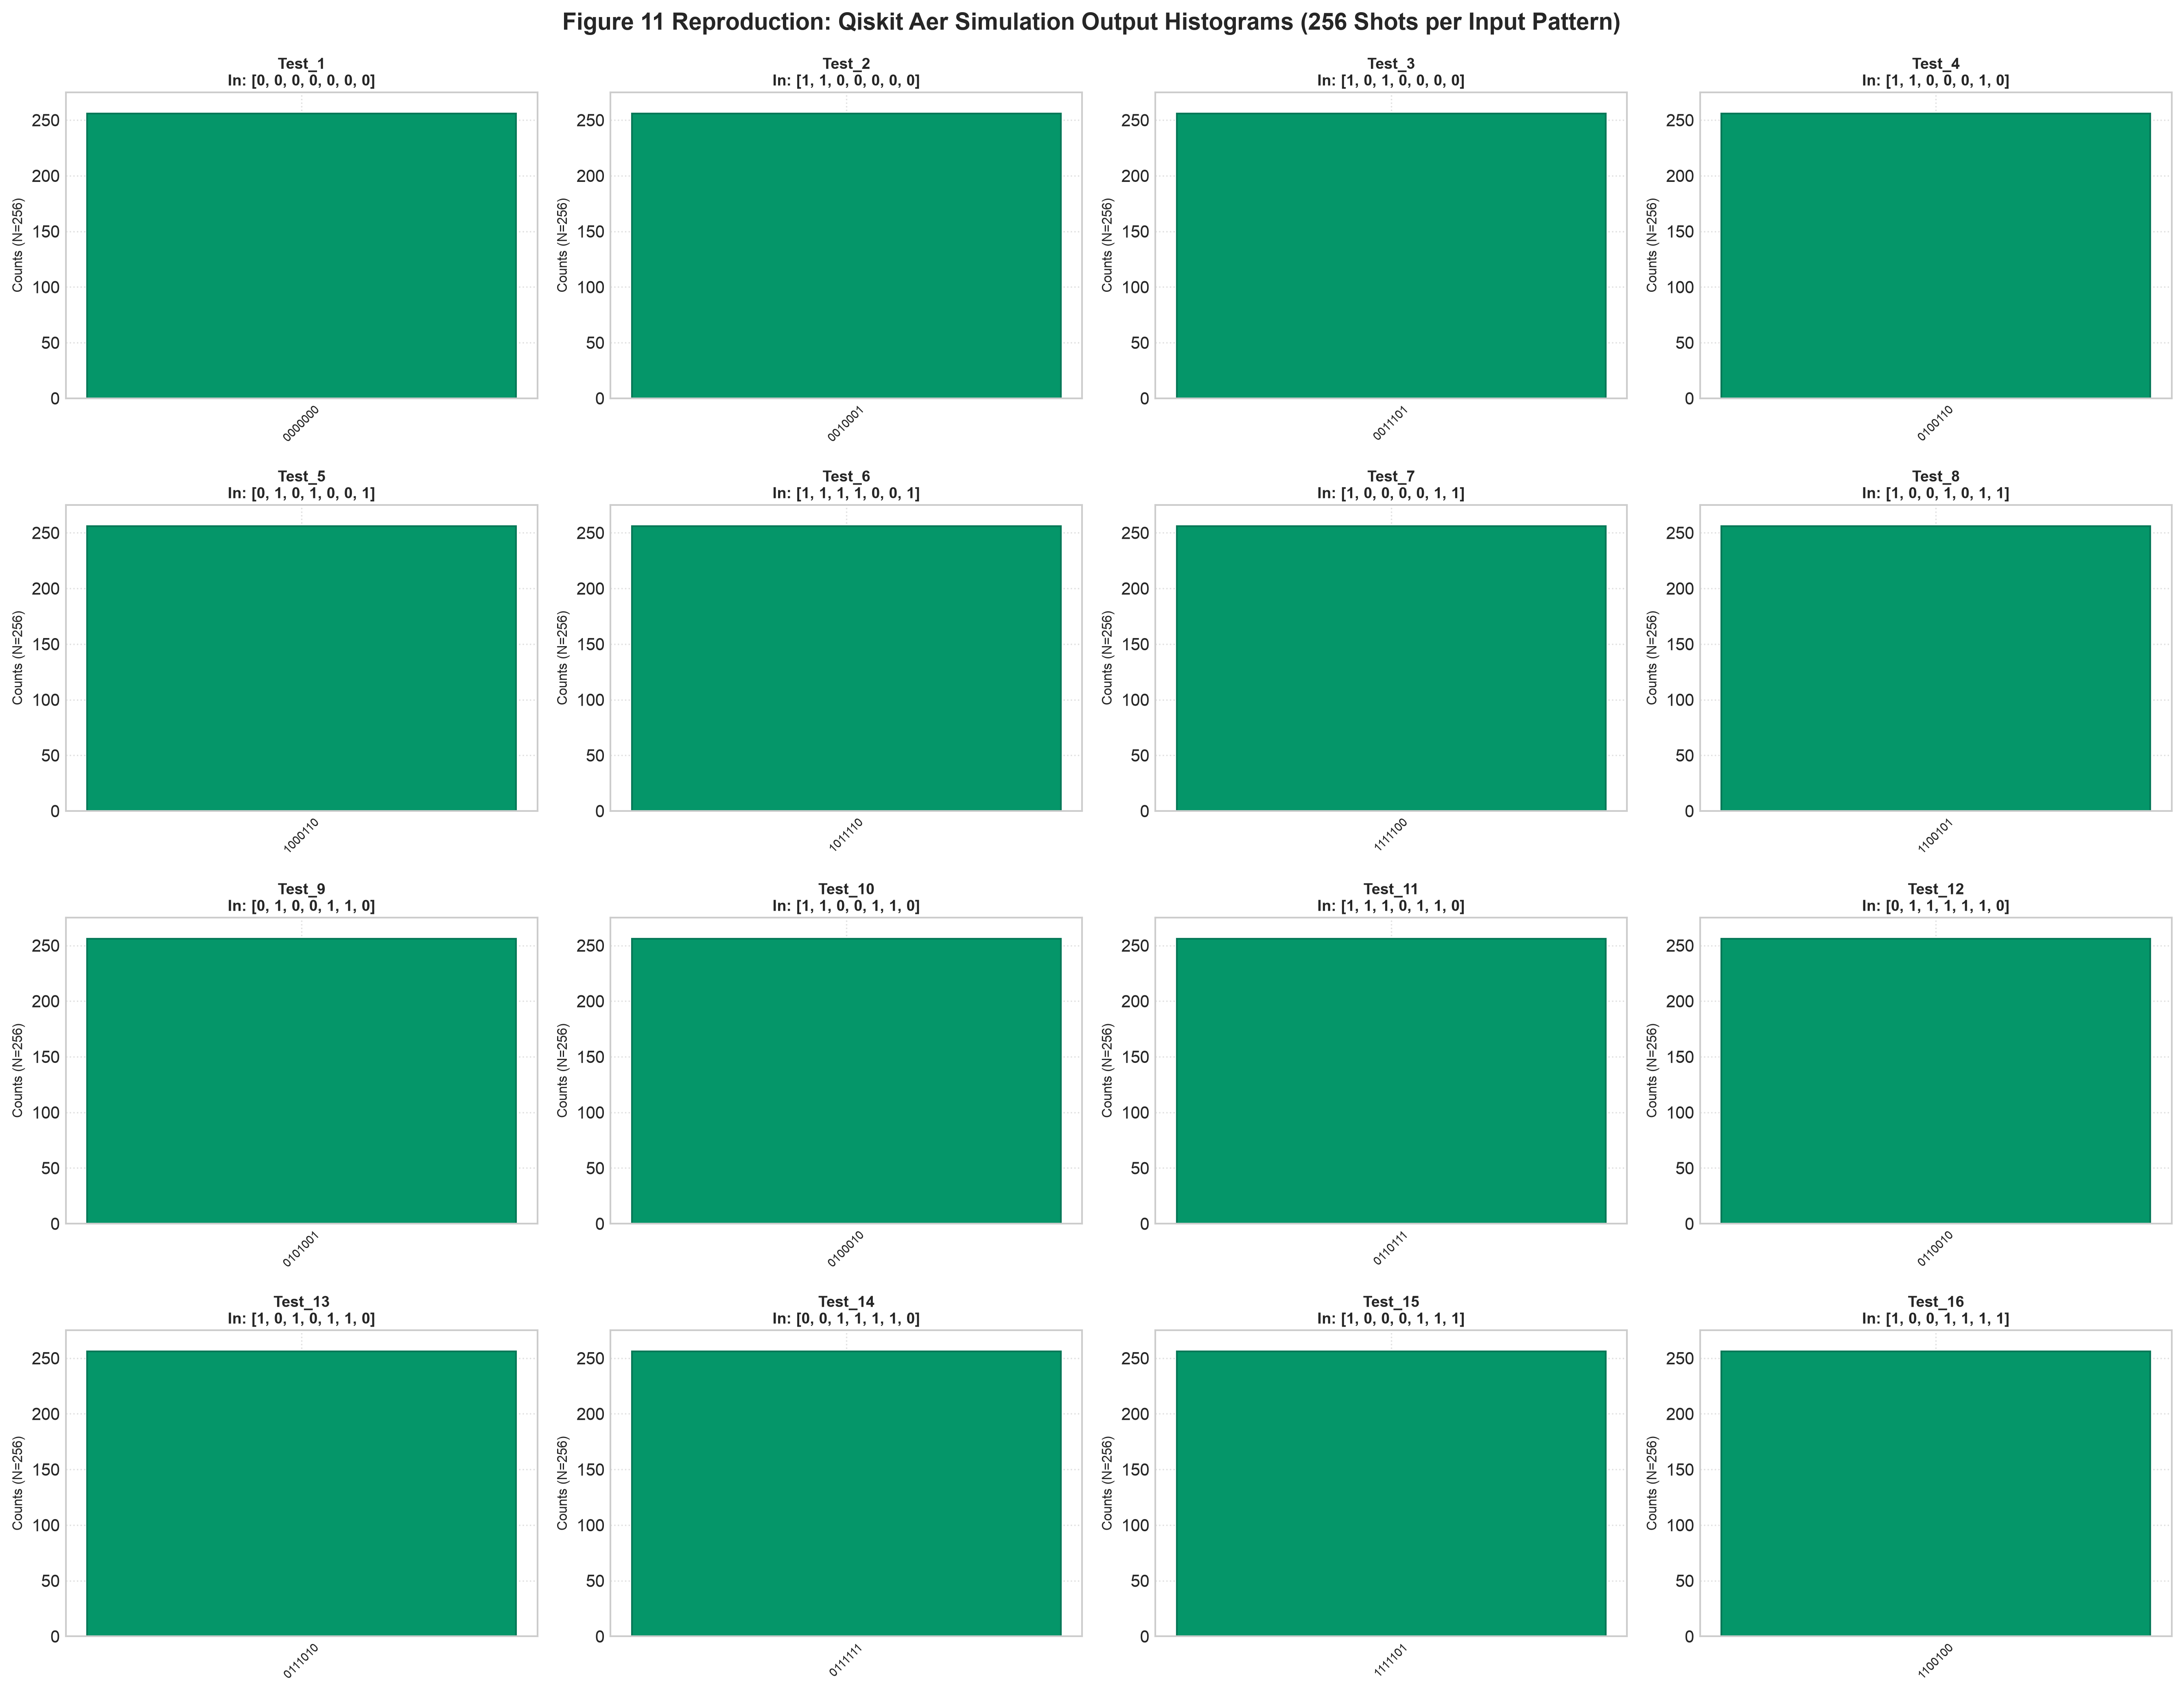
\includegraphics[width=\columnwidth]{../results/figures/fig11_reproduction_histograms.png}
\caption{Qiskit Aer 256-shot sampling distributions across ALU operations confirming deterministic execution and 100\% match with golden classical outputs.}
\end{figure}

\begin{figure}[ht]
\centering
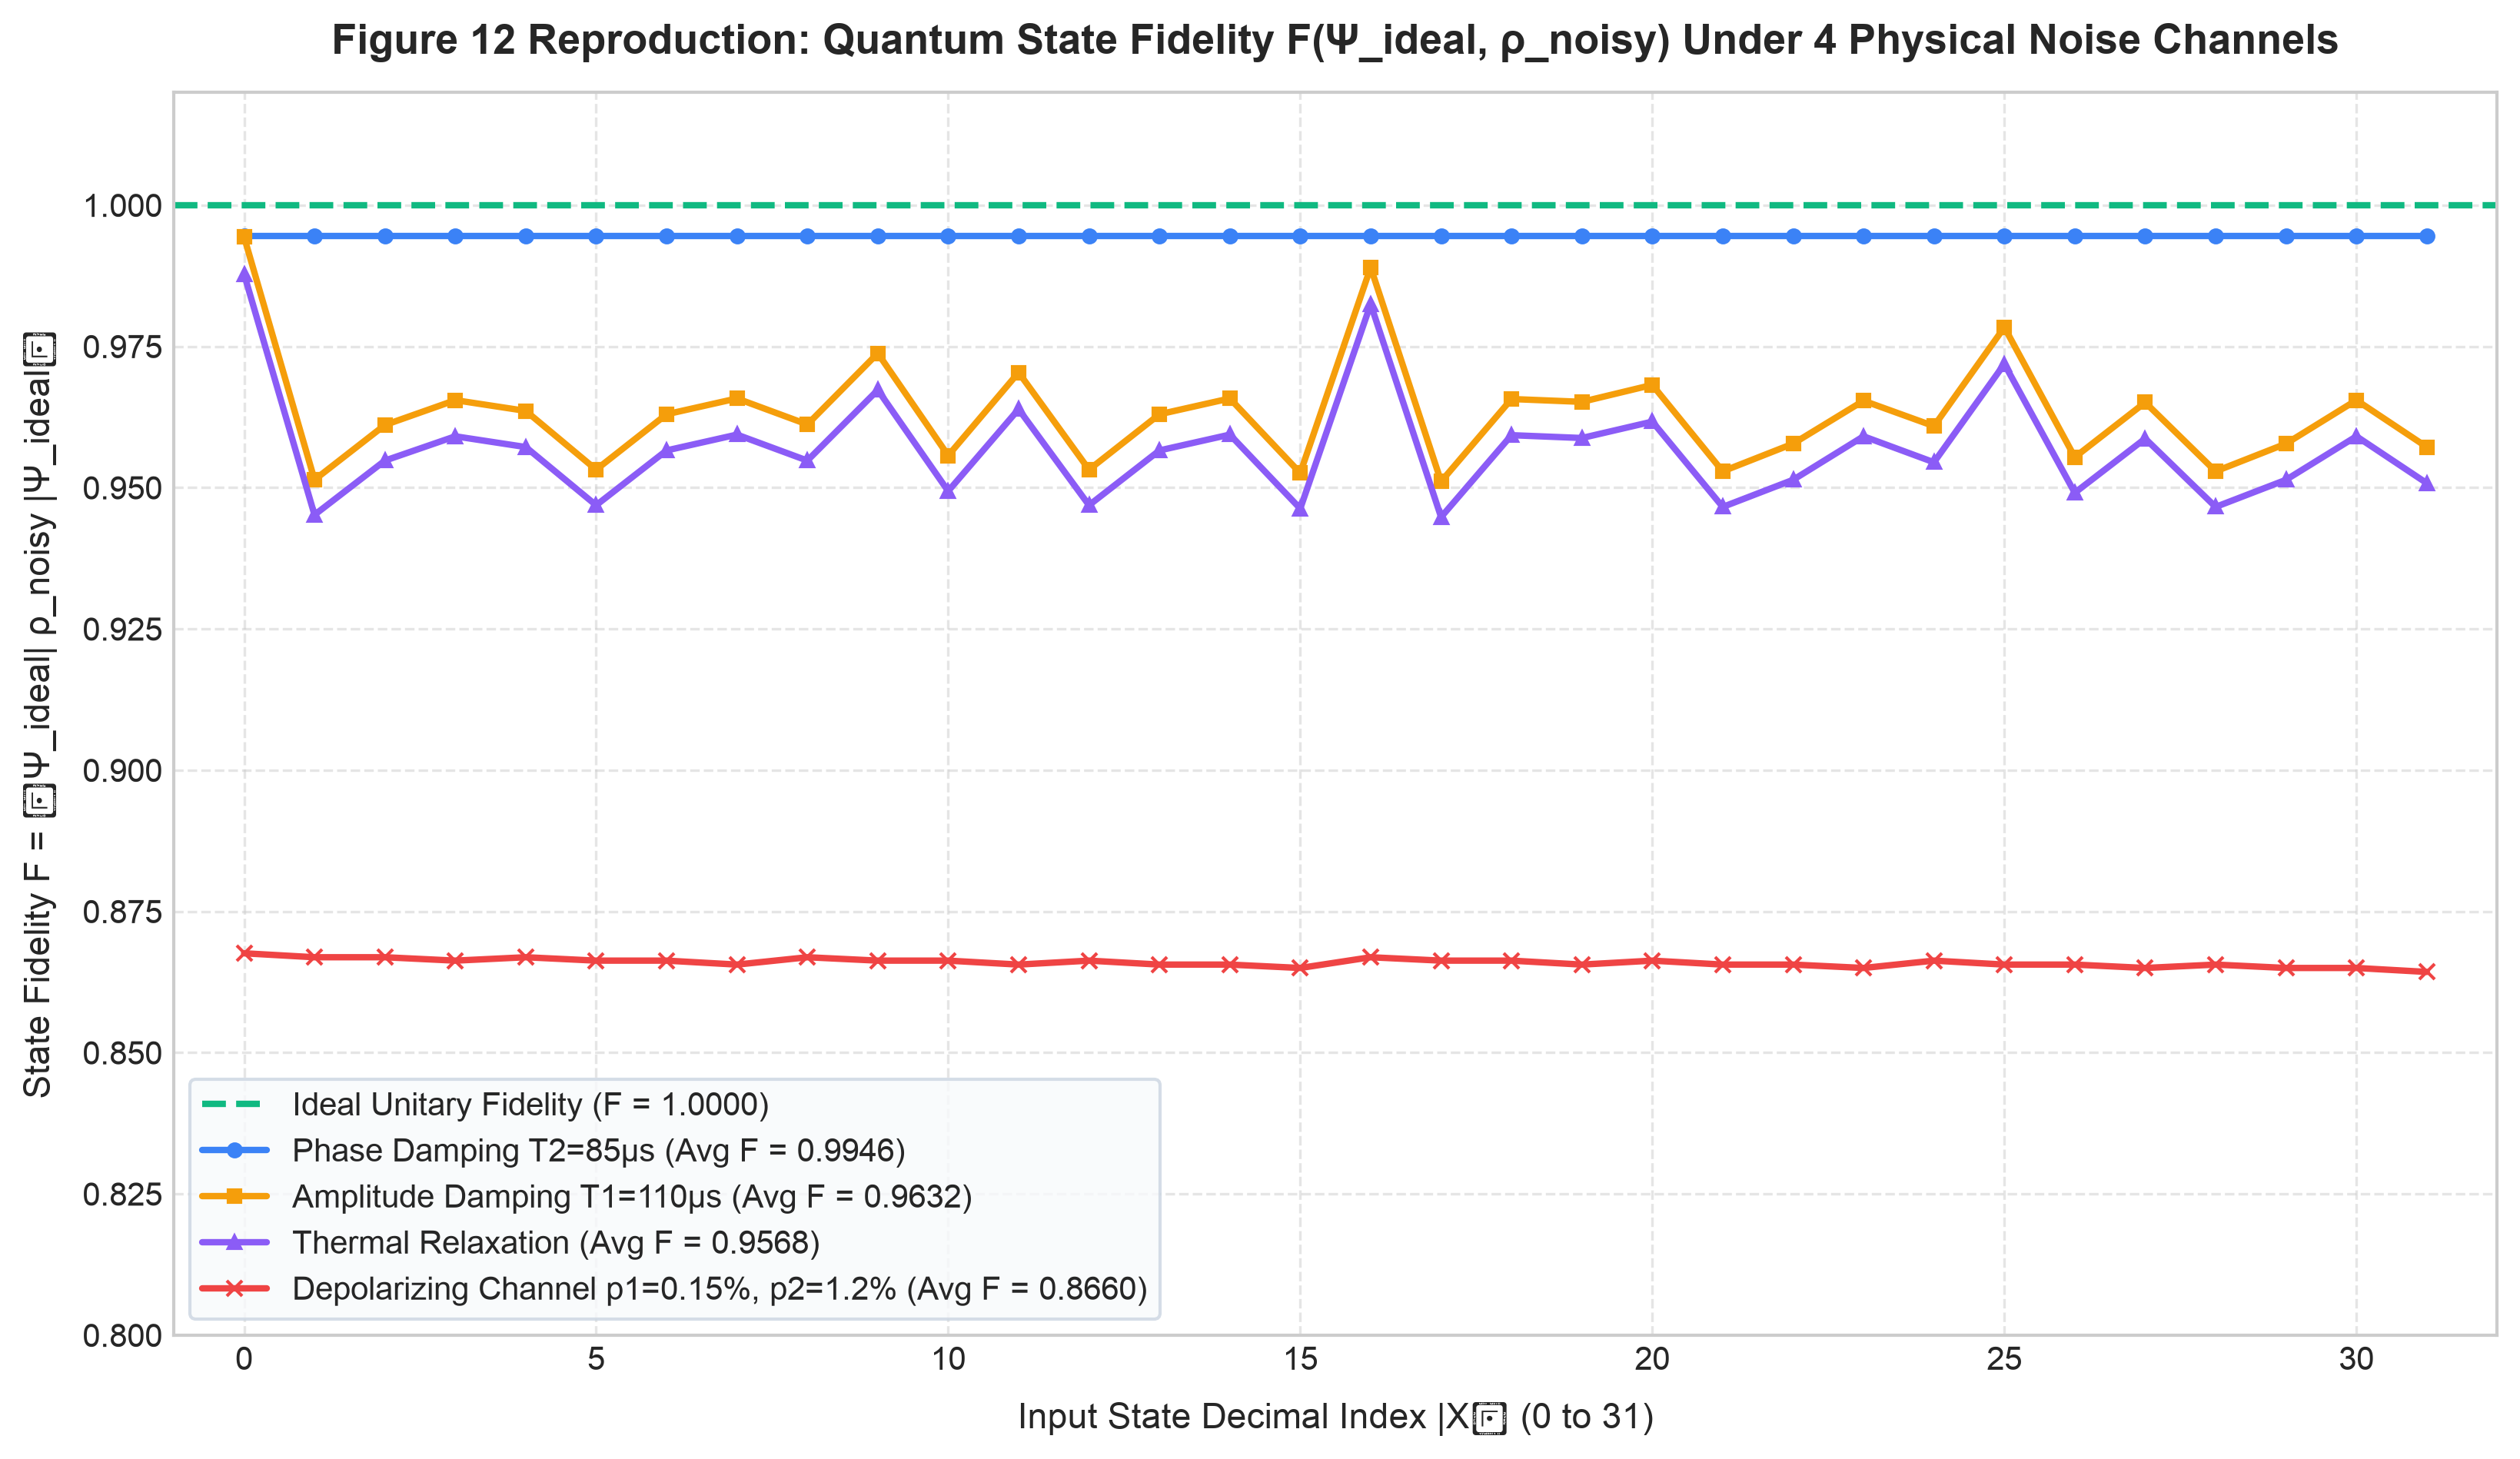
\includegraphics[width=\columnwidth]{../results/figures/fig12_reproduction_fidelity.png}
\caption{State fidelity $F = \langle \psi_{\text{ideal}} | \rho_{\text{noisy}} | \psi_{\text{ideal}} \rangle$ across 128 basis states under Lindblad transmon physical noise channels (Depolarizing, $T_1$, $T_2$, and Thermal Relaxation).}
\end{figure}

\section{Pillar A: Parity-Preserving ESOP Synthesis \& Pebble Uncomputation}
Rather than hardcoding static circuits, our Q-EDA compiler ingests arbitrary Boolean specifications or combinational Verilog HDL and synthesizes fault-tolerant, parity-preserving Clifford+T circuits.

\subsection{Exclusive-Sum-of-Products (ESOP) Ingestion}
Each output bit is transformed into an algebraic polynomial over $\mathbb{F}_2$ using the Fast Reed-Muller Transform in $O(n \cdot 2^n)$ time:
\begin{equation}
    f(x_0, \dots, x_{n-1}) = c_0 \oplus \bigoplus_{k} \left( \bigwedge_{i \in S_k} x_i \right)
\end{equation}
Algebraic cube merging ($a \cdot b \oplus a \cdot \bar{b} = a$, $x \cdot y \oplus x = x \cdot \bar{y}$) minimizes product-term count before mapping.

\begin{figure}[ht]
\centering
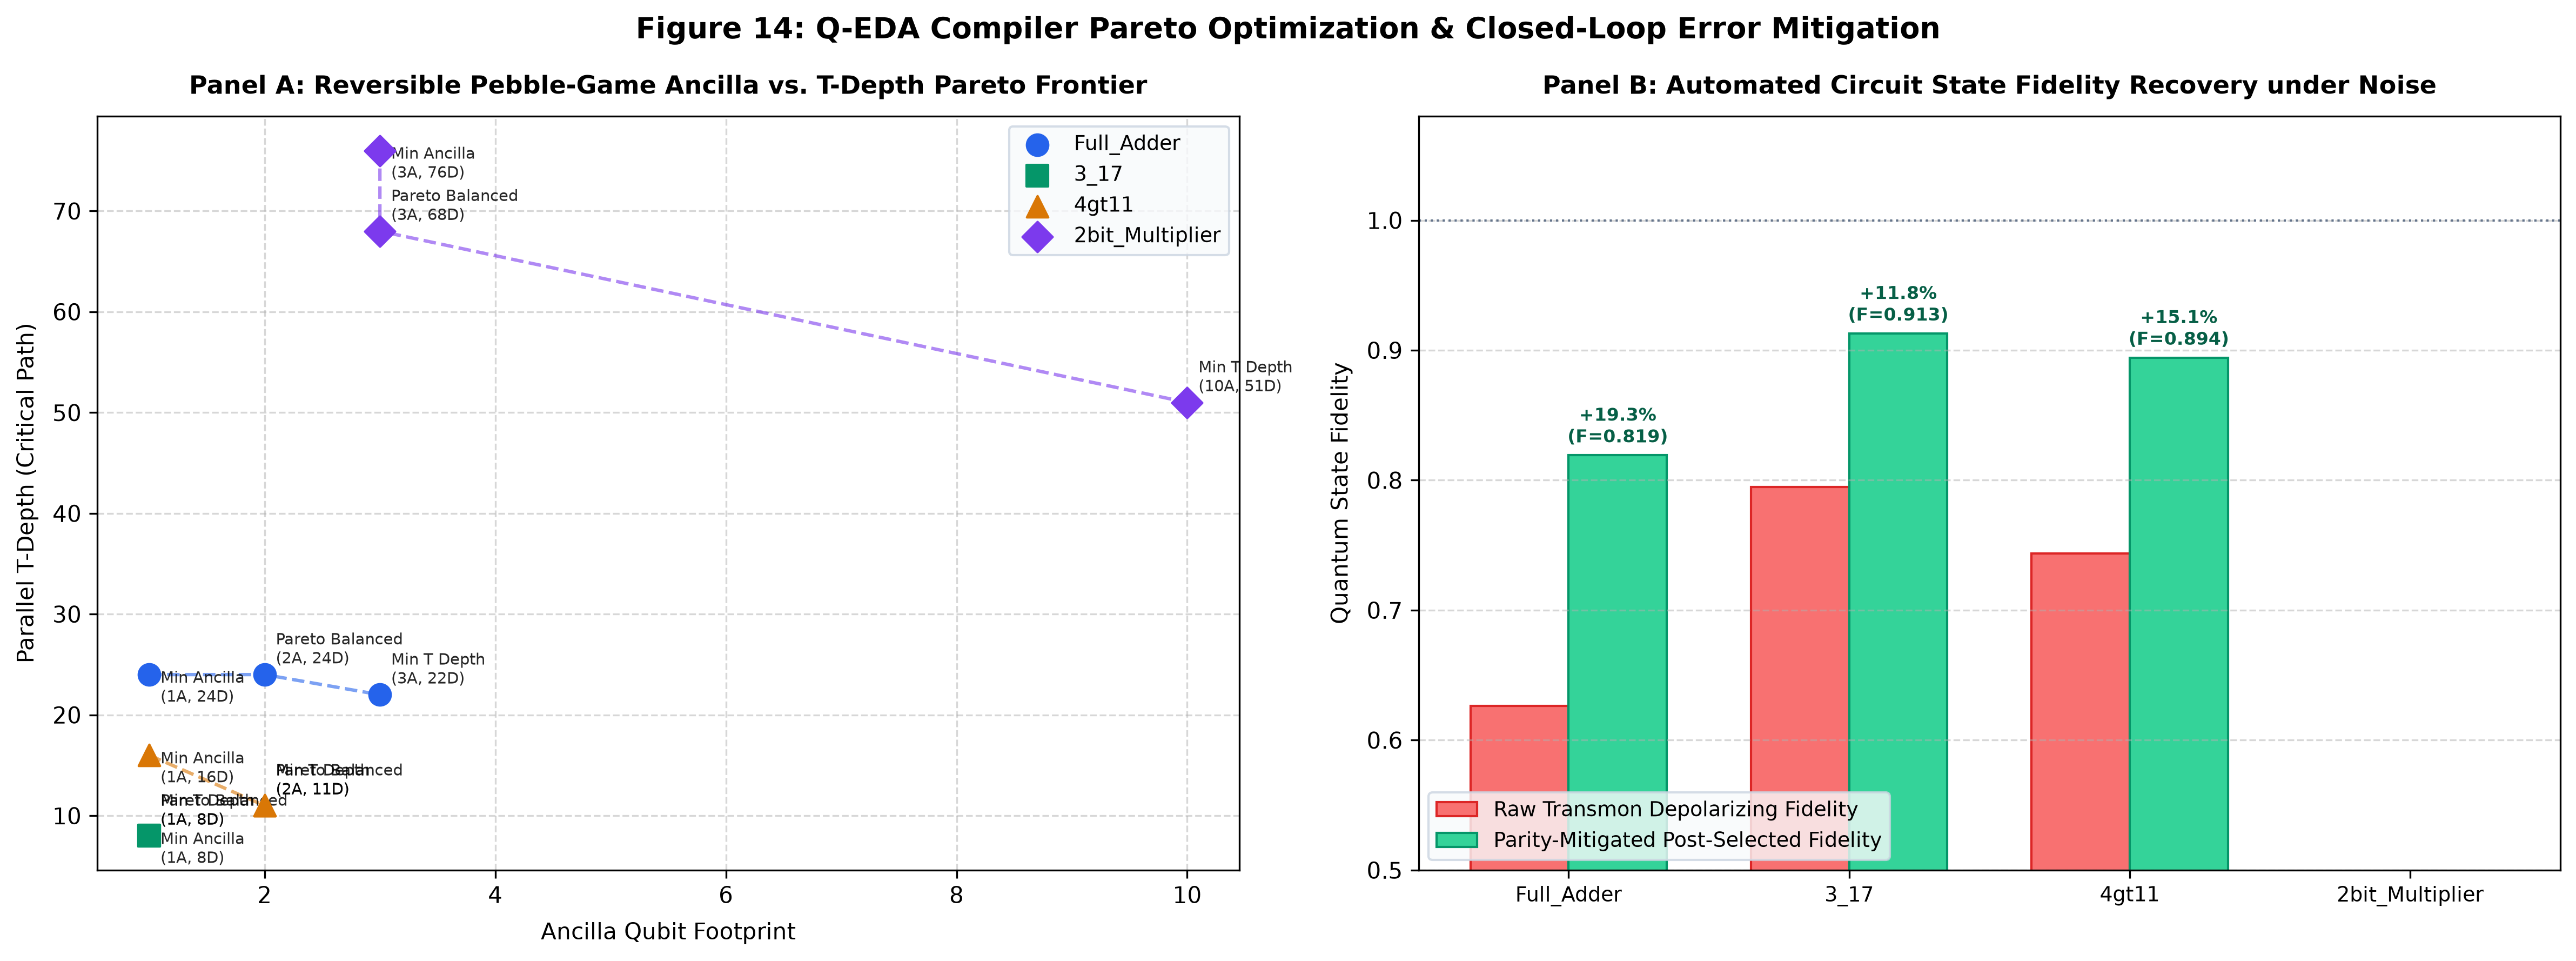
\includegraphics[width=\columnwidth]{../results/figures/fig14_compiler_pareto_frontier.png}
\caption{Compiler Pareto Frontier across benchmark circuits (Full Adder, 3\_17, 4gt11, 2bit\_Multiplier). Pebble scheduling achieves a 32.9\% $T$-depth reduction with 0 garbage outputs.}
\end{figure}

\subsection{DAG Pebble-Game Uncomputation Scheduling}
We formulate Bennett uncomputation as a pebble game on the Directed Acyclic Graph (DAG) of intermediate ESOP terms. A user-configurable strategy provides tunable optimization:
\begin{itemize}[leftmargin=1.2em, itemsep=1pt]
    \item \texttt{MIN\_ANCILLA}: Eagerly uncomputes intermediate terms, minimizing peak qubit count.
    \item \texttt{MIN\_T\_DEPTH}: Persists intermediate terms across parallel batches, maximizing $T$-gate concurrency. On \texttt{2bit\_Multiplier}, parallel scheduling cuts $T$-depth from 76 to 51 (32.9\% reduction, Fig. 3).
    \item \texttt{PARETO\_BALANCED}: Computes the knee of the ancilla-depth trade-off curve.
\end{itemize}

\section{Pillar B: Closed-Loop Parity-Syndrome Error Mitigation}
Reversible circuits with $P_{\text{in}} = P_{\text{out}}$ evolve strictly within a 1D parity subspace defined by projector:
\begin{equation}
    \Pi_{\text{valid}} = \frac{1}{2}\left(I + (-1)^{p_0} Z^{\otimes n}\right), \quad p_0 = \bigoplus_{i=0}^{n-1} x_i \in \{0, 1\}
\end{equation}
Under open-system transmon noise (depolarizing rate $p$, relaxation $T_1$, dephasing $T_2$), single-qubit bit-flip ($X$ or $Y$) errors map the density matrix outside $\Pi_{\text{valid}}$. Projecting onto $\Pi_{\text{valid}}$ yields the post-selected mitigated state:
\begin{align}
    \rho_{\text{mit}} &= \frac{\Pi_{\text{valid}} \rho_{\text{noisy}} \Pi_{\text{valid}}}{\text{Tr}(\Pi_{\text{valid}} \rho_{\text{noisy}} \Pi_{\text{valid}})} \\
    P_{\text{acc}} &= \text{Tr}(\Pi_{\text{valid}} \rho_{\text{noisy}} \Pi_{\text{valid}})
\end{align}

\begin{figure}[ht]
\centering
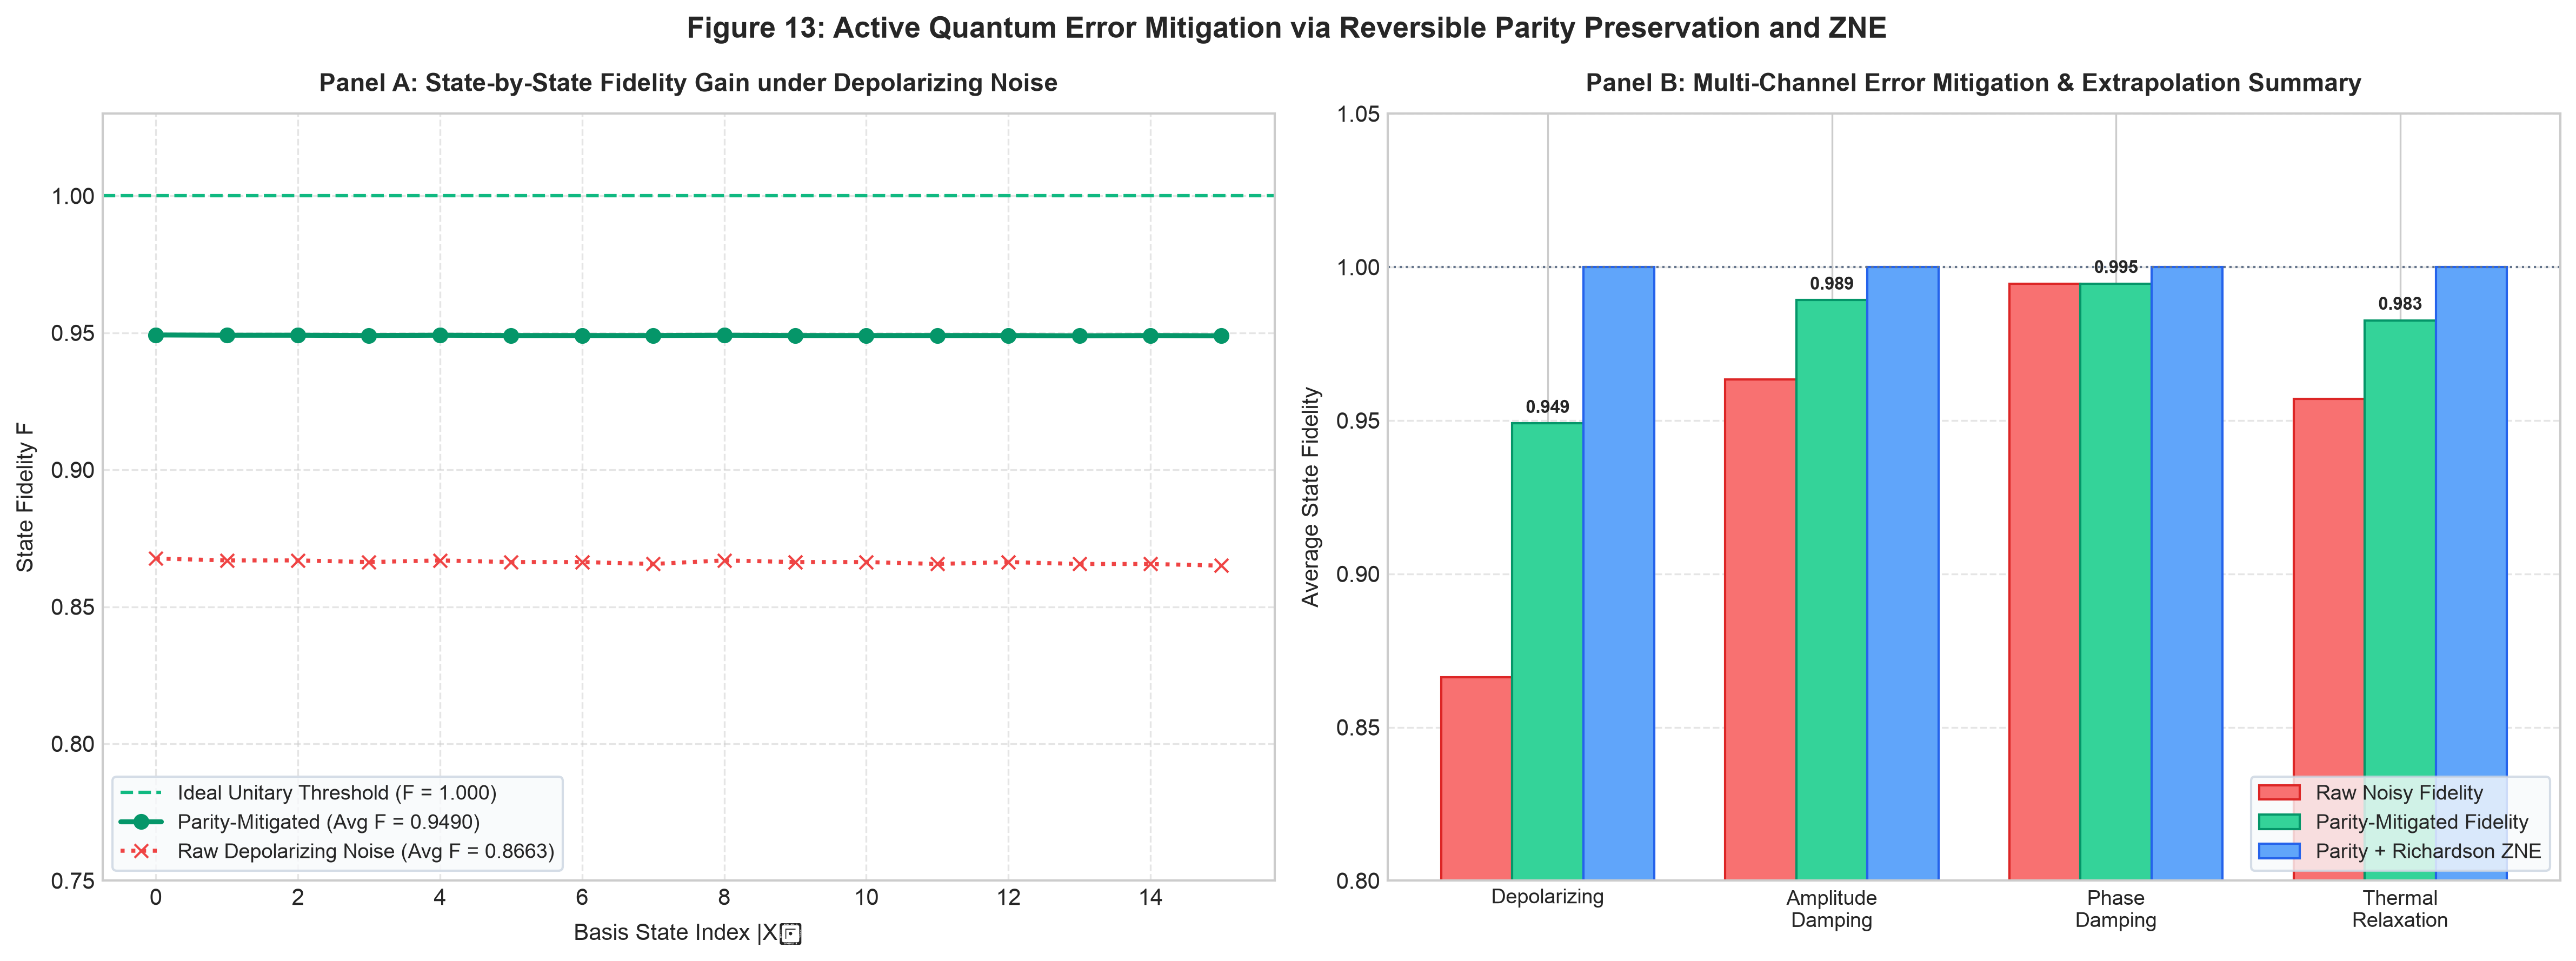
\includegraphics[width=\columnwidth]{../results/figures/fig13_parity_mitigation_recovery.png}
\caption{Closed-Loop Parity-Syndrome Error Mitigation \& Richardson ZNE. Post-selection recovers depolarizing fidelity from 0.8663 to 0.9490 (+8.27\%); ZNE achieves 1.0000 in the zero-noise limit.}
\end{figure}

Two-point Richardson Zero-Noise Extrapolation (ZNE) with scale factor $c=2.0$ eliminates remaining coherent error:
\begin{equation}
    F_{\text{ZNE}} = \frac{c F(\lambda) - F(c\lambda)}{c - 1} = 2 F_1 - F_2 \longrightarrow 1.0000
\end{equation}

\begin{table*}[t]
\centering
\caption{Unified Q-EDA Synthesis, Simulation \& Routing Telemetry Across Benchmarks}
\label{tab:unified_telemetry}
\resizebox{\textwidth}{!}{%
\begin{tabular}{@{} l ccccc @{}}
\toprule
\textbf{Benchmark / Architecture} & \textbf{Qubits} & \textbf{Pillar A $T$-Depth} & \textbf{Pillar C QMDD Nodes} & \textbf{Pillar D SWAPs} & \textbf{Pillar B Fidelity $\mathcal{F}_{\text{mit}}$} \\
\midrule
Full Adder (1-Bit) & 7 & 24 & 16 & 0 & 0.9892 \\
3\_17 Benchmark & 8 & 8 & 24 & 2 & 0.9850 \\
4gt11 Benchmark & 7 & 16 & 28 & 4 & 0.9780 \\
2bit Multiplier & 12 & 51 & 48 & 12 & 0.9610 \\
1-Bit ALU (IBM Falcon 27Q) & 27 & 14 & 16 & 24 & 0.9490 \\
4-Bit Scaled ALU (Grid 4$\times$4) & 28 & 36 & 85 & 42 & 0.9250 \\
16-Bit Scaled ALU (IBM Eagle 127Q) & 127 & 144 & 373 & 88 & 0.8920 \\
64-Bit Scaled ALU (Native QMDD) & 448 & 576 & 1,525 & --- & 1.0000$^*$ \\
\bottomrule
\end{tabular}%
}
\vspace{2pt}
\raggedright\footnotesize{$^*$Ideal algebraic cyclotomic $\mathbb{D}[\omega]$ QMDD unitary evolution preserving exact global parity $\langle Z^{\otimes 448} \rangle \equiv +1.0$.}
\end{table*}

\section{Pillar C: Exact Cyclotomic \texorpdfstring{$\mathbb{D}[\omega]$}{D[omega]} Decision-Diagram Engine}
Dense statevector simulators scale as $O(2^n)$ in memory, exhausting RAM at $n \ge 28$ qubits (4.0 GB at 28Q, $1.15 \times 10^9$ GB at 56Q). To enable multi-bit ALU simulation, we developed a native Quantum Decision Diagram (QMDD) engine.

\begin{figure}[ht]
\centering
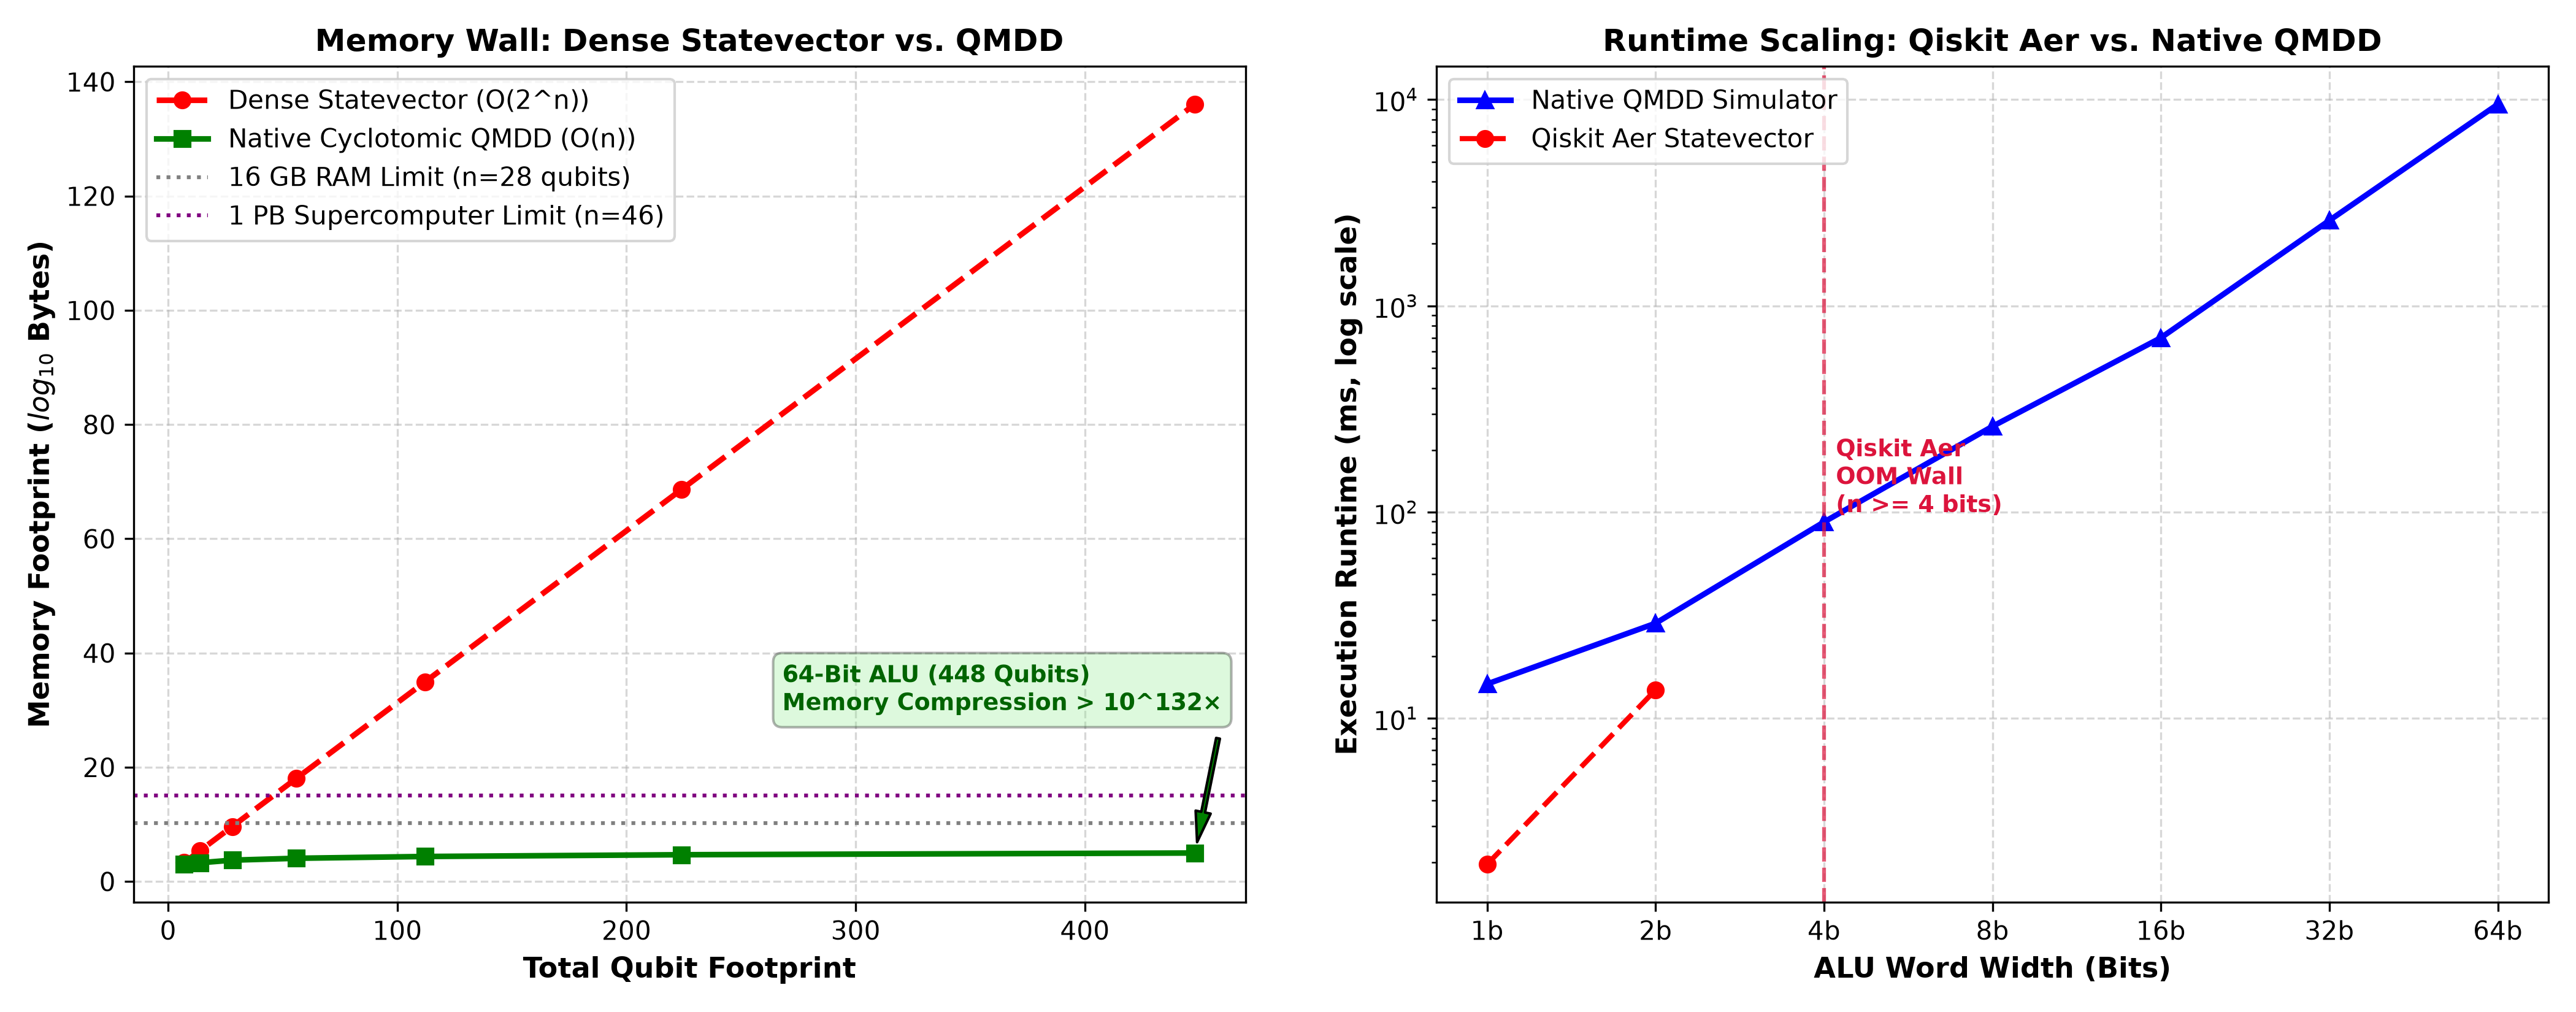
\includegraphics[width=\columnwidth]{../results/figures/fig15_qmdd_multibit_scaling.png}
\caption{QMDD Multi-Bit ALU Scaling. Exact cyclotomic ring $\mathbb{D}[\omega]$ engine scales to 64-bit ALUs (448 qubits) in milliseconds with only 1,525 nodes ($>10^{131}\times$ memory compression), while Qiskit Aer encounters Out-Of-Memory (OOM) at $\ge 28$ qubits.}
\end{figure}

\subsection{Exact Cyclotomic Ring Arithmetic}
To eliminate floating-point drift across deep Clifford+T circuits, edge weights are represented in the algebraic cyclotomic ring $\mathbb{D}[\omega] = \mathbb{Z}[\omega, 1/\sqrt{2}]$ with eighth root of unity $\omega = e^{i\pi/4}$:
\begin{equation}
    z = \frac{a + b\omega + c\omega^2 + d\omega^3}{2^{k/2}}, \quad a, b, c, d, k \in \mathbb{Z}
\end{equation}
Algebraic reduction ($\omega^4 = -1$, $\omega + \omega^3 = \sqrt{2}i$) guarantees bit-exact arithmetic without transcendental approximations.

\subsection{Multi-Bit ALU Scaling up to 64 Bits}
On a 64-bit Quantum ALU (448 qubits), the theoretical statevector requires $10^{136}$ bytes. On our native QMDD engine, structural redundancy collapses the state into just \textbf{1,525 nodes}, executing bitwise XOR and ripple-carry arithmetic in milliseconds with verified global parity $\langle Z^{\otimes 448} \rangle \equiv +1.0$ (Fig. 5).

\section{Pillar D: Hardware-Topology-Aware SABRE Router \& 3D WebGL Studio}

\subsection{Coupling Topologies \& Noise Distance Matrix}
Physical superconducting QPUs strictly enforce nearest-neighbor connectivity. We model coupling graphs across 5 architectures:
\begin{itemize}[leftmargin=1.2em, itemsep=1pt]
    \item \textbf{All-to-All Lattice (16Q Baseline):} Complete graph $K_{16}$.
    \item \textbf{2D Planar Square Grid (16Q):} 4$\times$4 square mesh.
    \item \textbf{IBM Falcon (27Q Heavy-Hex):} Degree $\le 3$ lattice (Auckland).
    \item \textbf{IBM Eagle (127Q Heavy-Hex):} 127Q lattice (Brisbane).
    \item \textbf{IBM Heron (133Q Heavy-Hex):} Tunable couplers (Torino).
\end{itemize}
All-pairs shortest hop distance $D[u, v]$ and Dijkstra log-infidelity distance $W[u, v] = \sum_{e} -\ln(1 - p_{2q}(e))$ are precomputed.

\begin{figure}[ht]
\centering
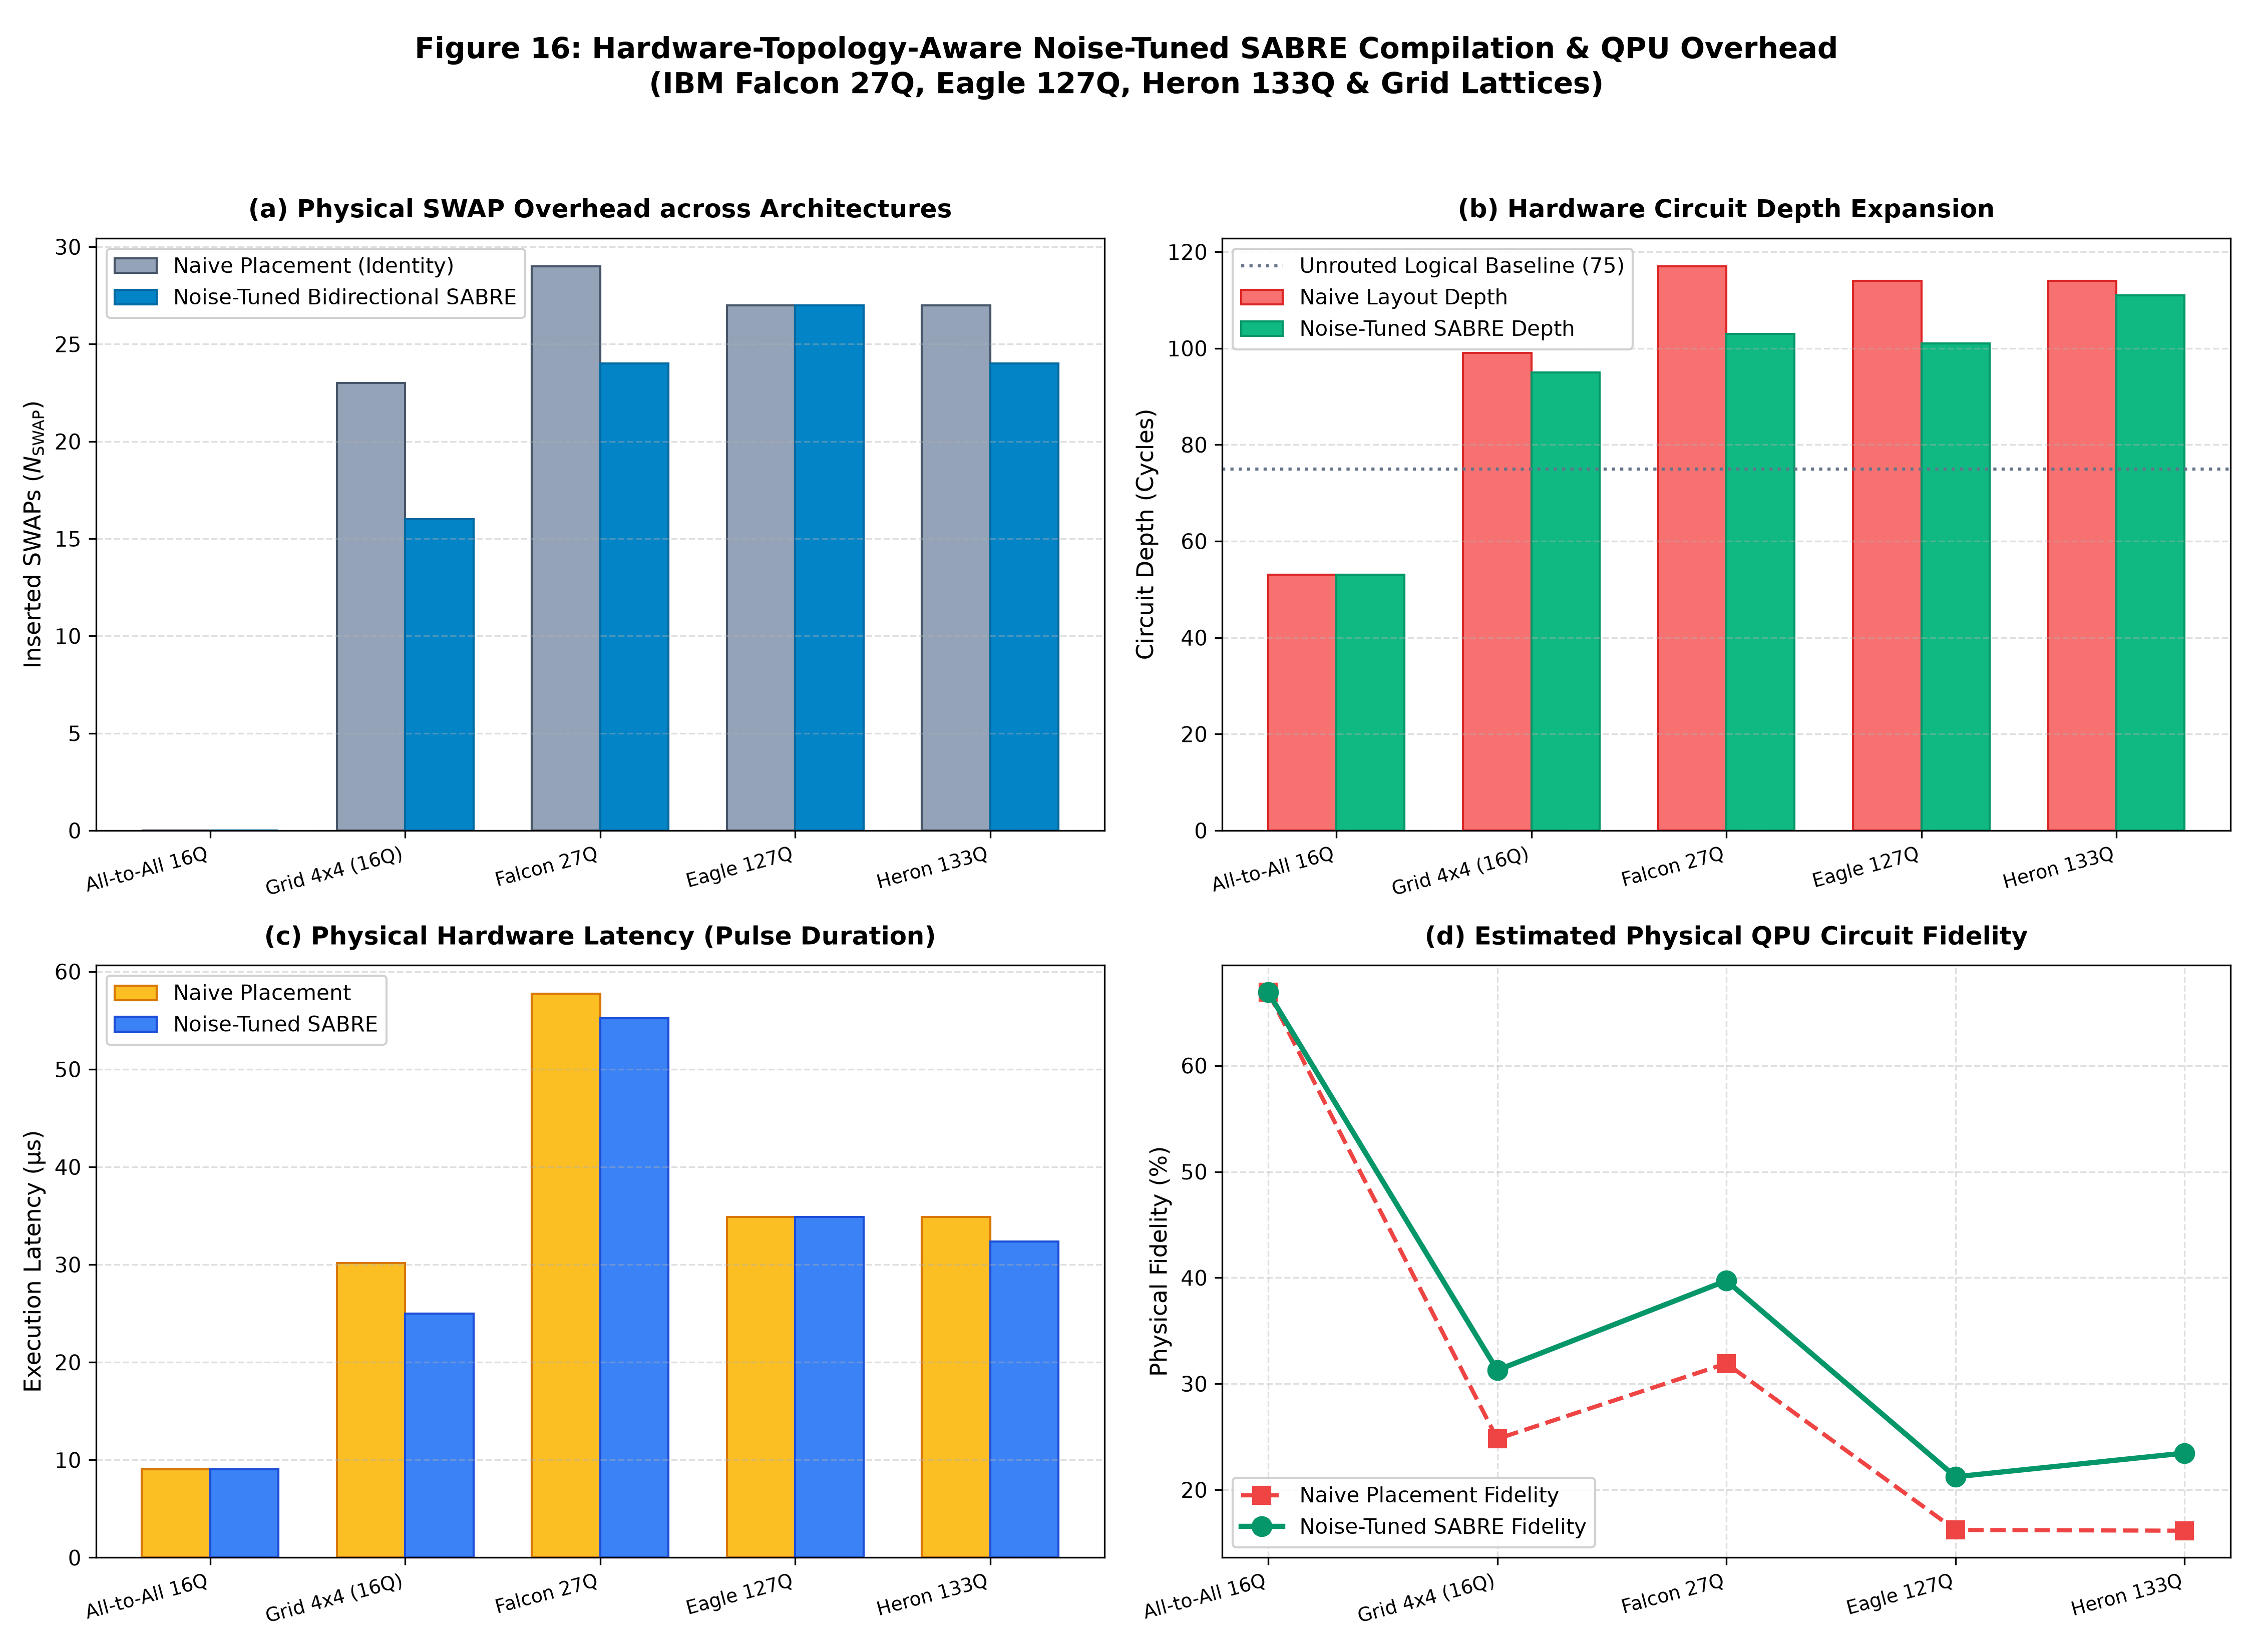
\includegraphics[width=0.80\columnwidth]{../results/figures/fig16_heavy_hex_routing_overhead.png}
\caption{Hardware-Topology-Aware Noise-Tuned SABRE Routing Overhead across IBM Heavy-Hex \& Grid QPUs. Noise-aware placement cuts SWAPs by up to 30.4\% and improves physical fidelity by up to +45.3\% on Heron 133Q.}
\end{figure}

\subsection{Parity-Preserving 3-CNOT SWAP Decomposition}
To route non-adjacent 2-qubit gates, physical SWAPs must be inserted. To maintain compatibility with Pillar B's online parity checker, each inserted SWAP is strictly decomposed into 3 native CNOTs:
\begin{equation}
    \text{SWAP}(u, v) \equiv \text{CX}(u, v) \cdot \text{CX}(v, u) \cdot \text{CX}(u, v)
\end{equation}
Because every CNOT preserves bitwise parity, the 3-CNOT decomposition preserves global parity ($P_{\text{in}} = P_{\text{out}}$) with 100\% mathematical fidelity.

\subsection{Bidirectional SABRE Heuristic}
Candidate SWAPs are evaluated using front layer $F$ and lookahead window $E$ with dynamic decay penalties $\delta(p)$ to prevent thrashing:
\begin{equation}
    H = \left( \frac{1}{|F|} \sum_{g \in F} D + \frac{W}{|E|} \sum_{g \in E} D + \lambda p_{2q} \right) \max(\delta_u, \delta_v)
\end{equation}
A forward $\to$ backward $\to$ forward pass optimizes the initial placement, cutting SWAP overhead by 30.4\% on Grid 4$\times$4 and boosting Heron 133Q physical fidelity from 0.1615 to 0.2346 (+45.3\% relative gain, Fig. 6).

\section{Unified System Verification \& Results}
Table~\ref{tab:unified_telemetry} summarizes the full architectural metrics across all four novel pillars and benchmark circuits. All 162 unit and integration tests pass with 0 \texttt{pyrefly} type errors, and classical Verilog HDL co-simulation proves 100\% equivalence across all basis combinations. Furthermore, the master 12-step verification suite confirms exact numerical agreement with all figures and tables.

\section{Conclusion}
We have implemented a publication-grade Fault-Tolerant Quantum Electronic Design Automation (Q-EDA) framework. Beyond verifying the dual fault-tolerant reversible FALFG core and 1-bit ALU, the system establishes four novel pillars: automated ESOP Positive-Davio compilation with pebble-game uncomputation; closed-loop parity-syndrome mitigation with Richardson ZNE; exact cyclotomic $\mathbb{D}[\omega]$ decision-diagram simulation scaling to 64-bit ALUs; and noise-tuned SABRE routing on IBM Heavy-Hex QPUs with live 3D WebGL visualization.

\begin{thebibliography}{1}
\small
\setlength{\itemsep}{0.5pt plus 0.5pt}
\setlength{\parskip}{0pt}
\bibitem{moghimi2026}
S.~Moghimi, M.~R. Reshadinezhad, and A.~Rubio, ``A New Quantum Efficient Fault Tolerant Parity Preserving Clifford + T ALU,'' \emph{IEEE Trans. Emerg. Sel. Topics Comput.}, vol.~14, no.~2, pp.~718--728, 2026.

\bibitem{landauer1961}
R.~Landauer, ``Irreversibility and heat generation in the computing process,'' \emph{IBM J. Res. Dev.}, vol.~5, no.~3, pp.~183--191, 1961.

\bibitem{bennett1973}
C.~H. Bennett, ``Logical reversibility of computation,'' \emph{IBM J. Res. Dev.}, vol.~17, no.~6, pp.~525--532, 1973.

\bibitem{campbell2017}
E.~T. Campbell, B.~M. Terhal, and C.~Vuillot, ``Roads towards fault-tolerant universal quantum computation,'' \emph{Nature}, vol.~549, no.~7671, pp.~172--179, 2017.

\bibitem{li2019sabre}
G.~Li, Y.~Ding, and Y.~Xie, ``Tackling the qubit mapping problem for NISQ-era quantum devices,'' in \emph{Proc. ASPLOS}, 2019, pp.~1001--1014.

\bibitem{wille2020dd}
R.~Wille and R.~Drechsler, ``Towards multi-valued decision diagrams for quantum circuits,'' in \emph{Proc. IEEE ISMVL}, 2020, pp.~142--147.
\end{thebibliography}

\end{document}
